\chapter{Introduction to ordinal numbers with the Coq proof assistant}

In this chapter, we introduce on  simple examples the main concepts which are developped later.  We assume the reader to have a very basic experience with the \coq{} proof assistant, for instance with one of the numerous tutorials one can consult on Internet
(see for instance \url{https://coq.inria.fr/documentation}). A basic experience  with Peano numbers (library \texttt{Arith}) would be useful.

The definitions  and theorems we are going to show are just simpler versions (\emph{i.e.} restrictions) of the ones contained in the forthcoming chapters. We hope that this simplicity will help to understand how we represent, compute and reason about ordinal notations.



\section{Ordinal numbers}
\index{Maths!Ordinal numbers}

The proof of termination of all hydra battles presented in~\cite{KP82} is based
on \emph{ordinal numbers}.
From a mathematical point of view, an ordinal is a representant of an equivalence class for isomorphims of strict, total and well-founded orders.

We can also associate to every ordinal $\alpha$ a set whose elements are all ordinals strictly less than $\alpha$. Thus, it is meaningful  to consider \emph{finite}, \emph{infinite}, \emph{demunerable} and \emph{non-countable} ordinals.
The relation $<$ on ordinals is well-founded, and the order $\leq$ associated with
$<$ is total.

We cannot cite all the litterature published on ordinals since Cantor's book 
\cite{cantorbook}, and 
leave it to the reader to explore the bibliography. Let us cite the book by Schütte~\cite{schutte} which contains an axiomatic definition of the set of countable ordinals we used as a mathematical specification of our implementaion in \coq{}~\cite{CantorContrib}. 


Out of respect of the tradition, the meta-variables for ordinals will be 
 $\alpha$, $\beta$, $\gamma$, etc. 

\subsection{Definitions}

\begin{itemize}
\item Let  $\alpha$ be an ordinal; we say that  $\alpha$ is a \emph{successor} if there exists some ordinal  $\beta$ such that 
$\alpha$ is is the least ordinal strictly greater than  $\beta$.

\item We say that an ordinal $\lambda$ is a \emph{limit ordinal} is $\lambda$  is the least upper bound of a stricly increasing sequence of ordinals.
The meta-variable $\lambda$ will be used for denoting  limit ordinals.

\item \index{Maths!Transfinite induction}
An ordinal is either $0$, a limit ordinal or a successor ordinal. This case analysis, as well as \emph{transfinite} ({i.e.}, well-founded) induction is used in many proofs about ordinal numbers.

\item Let $\alpha$ be any ordinal, the \emph{segment} $\mathbb{O}_\alpha$ is the
interval $[0,\alpha[\,=\,\{\beta|0\leq\beta<\alpha\}$. 

\item The set  of finite ordinals is a segment isomorphic to the set of natural numbers.
 The first infinite ordinal is the limit ordinal $\omega$.
 
\item The operations $+$, $\times$ and exponentiation on $\mathbb{N}$ are extended on ordinals numbers. Note that these  extensions are not commutative any more.  For instance $\omega = 1 + \omega \not= \omega + 1$
and $\omega = 2 \times \omega \not= \omega \times 2$.

\item The ordinal $\epsilon_0$ is the least solution of the equation
 \(\alpha=\omega^{\alpha}\).
\end{itemize}


Please note that the set of countable ordinals is not countable. 

Without ambiguity we will often denote the segment $\mathbb{O}_\alpha$ by just $\alpha$.
 


\section{Ordinal notations}
In a proof assistant like \coq{},  it is useful to represent ordinals through some data-type, and make arithmetical operations and comparison effectively implemented  through certified functions.

Of course, since the set of all countable ordinals is not countable, it cannot be represented by a language of finite terms. So, we will study ordinal notations just  for countable segments.

\subsection{A type class for ordinal notations}

Let $<$ be some relation on a given type $A$. In order to build an ordinal  notation 
system out of $(A,<)$, we require $<$ to be a strict, well-founded order, and that 
the reflexive closure of $<$ is a total order on $A$.

\index{Coq!Techniques!Type classes}

Using \coq's standard library and type classes, we propose the following definition.

\vspace{4pt}
\noindent\emph{From Module~\href{../src/html/hydras.Prelude.Ordinal_generic.html}{Prelude.Ordinal\_generic}}

\begin{Coqsrc}
Class OrdinalNotation {A:Type}{lt: relation A}(sto:StrictOrder lt)
      (compare : A -> A -> comparison) :=
  { compare_correct :
      forall alpha beta:A,
        CompareSpec (alpha=beta) (lt alpha beta) (lt beta alpha)
                                 (compare alpha beta);
    wf : well_founded lt}.  
\end{Coqsrc}




\subsection{Notation systems for some small ordinals}

The following enumeration  shows  popular notation systems for several ordinals (shown in increasing order with respect to inclusion), and their possible representation in \coq{}.
Please keep in mind that a notation system for a given ordinal $\alpha$ represents 
ordinals \emph{strictly below} $\alpha$.

\subsubsection{Finite ordinals}
Let $n$ be some natural number. The segment associated with $n$ is the interval 
$[0,n[\,=\,\{0,1,\dots,n-1\}$. 

One may represent the ordinal $n$ by a sigma type.


\vspace{4pt}
\noindent\emph{From Module~\href{../src/html/hydras.Prelude.Finite_ordinals.html}{Prelude.Finite\_ordinals}}

\label{def: Finite-ord-type}
\begin{Coqsrc}
Coercion is_true: bool >-> Sortclass.

Definition t (n:nat) := {i:nat | Nat.ltb i  n}.
\end{Coqsrc}

The order on type \texttt{t $n$} is defined through the projection on \texttt{nat}.


\begin{Coqsrc}
Definition lt {n:nat} : relation (t n) :=
  fun alpha beta => Nat.ltb ( proj1_sig alpha) (proj1_sig beta).
\end{Coqsrc}

For instance, let us build two elements of the segment $[0, 7[$, \emph{i.e.} two
inhabitants of   type (\texttt{t 7}), and prove a simple  inequality (see Fig.~\ref{fig:O7}).

\begin{figure}[h]
\centering
\begin{tikzpicture}[very thick, scale=0.6]

\node (N0) at (0,0) {$\bullet$};
\node (i0) at (0,1) {$0$};
\node (N1) at (2,0) {$\bullet$};
\node (i1) at (2,1) {$1$};
\node (N2) at (4,0) {$\bullet$};
\node (i2) at (4,1) {$2$};
\node (N3) at (6,0) {$\bullet$};
\node (i3) at (6,1) {$3$};
\node (N4) at (8,0) {$\bullet$};
\node (i4) at (8,1) {$4$};
\node (N5) at (10,0) {$\bullet$};
\node (i5) at (10,1) {$5$};
\node (N6) at (12,0) {$\bullet$};
\node (i6) at (12,1) {$6$};
\node(alpha1) at (4,-1) {$\alpha_1$};
\node(alpha2) at (10,-1) {$\beta_1$};
\end{tikzpicture}

\caption{The segment $\mathbb{O}_7$\label{fig:O7}}
\end{figure}
  
\index{Coq!Commands!Program Definition}

\begin{Coqsrc}
Program Example alpha1 : t 7 := 2.

Program Example beta1 : t 7 := 5.

Example i1 : lt  alpha1 beta1.
Proof.   now compute. Qed.
\end{Coqsrc}




Note that the type \texttt{t 0} is empty, and that \texttt{Program} generates an obligation
for verifying that the constraint $i<n$ is fullfilled when one tries to build the $i$-th ordinal in type \texttt{t $n$}.

\begin{Coqsrc}
Lemma t0_empty (alpha: t 0): False.
Proof.
  destruct alpha.
  destruct x; cbn in i; discriminate.
Qed.


Program Definition bad : t 10 := 10.
Next Obligation.
  compute.
\end{Coqsrc}

\begin{Coqanswer}
1 subgoal (ID 162)
  
  ============================
  false = true
\end{Coqanswer}

\begin{Coqsrc}
Abort.
\end{Coqsrc}

Note also that attempting to compare an ordinal of type \texttt{t $n$}  with an ordinal of
type \texttt{t $p$}  leads to an error if $n$ and $p$ are not convertible.

\begin{Coqsrc}

Program Example gamma1 : t 8 := 7.

Fail Goal lt alpha1 gamma1.
\end{Coqsrc}

\begin{Coqanswer}
 The command has indeed failed with message:
The term "gamma1" has type "t 8" while it is expected to have type "t 7".
\end{Coqanswer}


In order to build an instance of \texttt{OrdinalNotation}, we define a comparison function, by delegation to standard library's  \texttt{Nat.compare}, and prove its correction.

\begin{Coqsrc}
Definition compare {n:nat} (alpha beta : t n) :=
  Nat.compare (proj1_sig alpha) (proj1_sig beta).

Lemma compare_correct {n} (alpha beta : t n) :
  CompareSpec (alpha = beta) (lt alpha beta) (lt beta alpha)
              (compare alpha beta).
\end{Coqsrc}

\begin{remark}
 The proof of \texttt{compare\_correct} uses a well-know pattern of \coq{}.
Let us consider  the following subgoal.

\begin{Coqanswer}
 1 subgoal (ID 110)
  
  n, x0 : nat
  i, i0 : x0 <? S n
  ============================
  exist (fun i1 : nat => i1 <=? n) x0 i =
  exist (fun i1 : nat => i1 <=? n) x0 i0
\end{Coqanswer}

Applying the tactic \texttt{f\_equal} generates a simpler subgoal.

\begin{Coqanswer}
1 subgoal (ID 112)
  
  n, x0 : nat
  i, i0 : x0 <? S n
  ============================
  i = i0
\end{Coqanswer}

We have now to prove that two proofs of \texttt{Nat.ltb x0 (S n)} are equal.

This is not obvious, but  a consequence of the following lemma of library 
\href{https://coq.inria.fr/distrib/current/stdlib/Coq.Logic.Eqdep_dec.html}{Coq.Logic.Eqdep\_dec}.

\index{Coq!Techniques!Unicity of equality proofs}

\begin{Coqanswer}
eq_proofs_unicity_on :
forall (A : Type) (x : A),
(forall y : A, x = y \/ x <> y) -> forall (y : A) (p1 p2 : x = y), p1 = p2
\end{Coqanswer}

Thus unicity of proofs of \texttt{Nat.ltb x0 (S n)}  comes from the decidability of
equality on type \texttt{bool}.

This is why we used the boolean function \texttt{Nat.ltb} instead of the inductive predicate \texttt{Nat.lt} in the definition of type \texttt{t $n$} (see page~\pageref{def: Finite-ord-type}).

For more information about this pattern, please lokk at the numerous mailing lists and 
FAQs on \coq{}).



\end{remark}


Applying lemmas of the libraries \texttt{Coq.Wellfounded.Inverse\_Image},
 \texttt{Coq.Wellfounded.Inclusion}, and \texttt{Coq.Arith.Wf\_nat}, we prove that our
relation \texttt{wf} is well founded.

\begin{Coqsrc}
Lemma lt_wf (n:nat) : well_founded (@lt n).
\end{Coqsrc}

Now we can build our instance of \texttt{OrdinalNotation}.

\begin{Coqsrc}
Global Instance sto n : StrictOrder (@lt n).

Global Instance FinOrd (n:nat) : OrdinalNotation (sto n) compare.
Proof.
  split.
  - apply compare_correct.
  - apply lt_wf.
Qed.
\end{Coqsrc}

Finally, it is interesting to show that the segment $[0,n[$ is a ``sub-segment'' of
$[0,n+1[$. Since types $t\;n$ are $t\;(n+1)$ are not convertible, we consider a ``cast'' 
function $\iota$ from $t\;n$ to $t\;(n+1)$, and prove this function is  a bijection  from $t\;n$ to
the segment $[0,n-1[$ of $t\;(n+1)$.



This notion is defined generically as a class in
 Module~\href{../src/html/hydras.Prelude.Ordinal-generic.html}{Prelude.Ordinal\_generic} (see Fig~\vref{figure:subsegment}).

\begin{Coqsrc}
(** The segment associated with nA is isomorphic to
    the interval [0,b[ *)

Class  Subsegment 
       `(nA : @OrdinalNotation A ltA stoA compareA)
       `(nB : @OrdinalNotation B ltB stoB compareB)
       (b :  B)
       (iota : A -> B):=
  {
  subseg_compare :forall x y : A,  compareB (iota x) (iota y) =
                                 compareA x y;
  subseg_incl : forall x, ltB (iota x) b;
  subseg_onto : forall y, ltB y b  -> exists x:A, iota x = y}.
\end{Coqsrc}


 \begin{figure}[h]
   \centering
   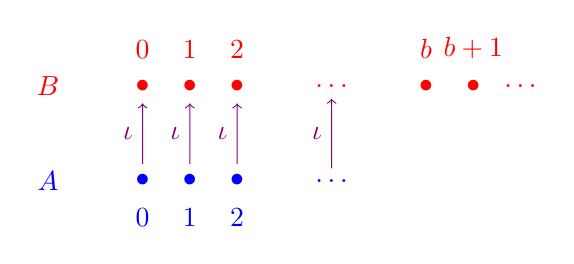
\begin{tikzpicture}[very thick, scale=0.6]
\begin{scope}[color=blue]
\node (A) at (0,0) {$A$};
\node(A0) at (2,0)[label=below:$0$]{$\bullet$};
\node(A1) at (3,0)[label=below:$1$]{$\bullet$};
\node(A2) at (4,0)[label=below:$2$]{$\bullet$};
\node (Adots) at (6,0) {$\ldots$};
\end{scope}
\begin{scope}[color=red]
\node (B) at (0,2) {$B$};
\node(B0) at (2,2)[label=above:$0$]{$\bullet$};
\node(B1) at (3,2)[label=above:$1$]{$\bullet$};
\node(B2) at (4,2)[label=above:$2$]{$\bullet$};
\node (Bdots) at (6,2) {$\ldots$};
\node (b) at (8,2) [label=above:$b$]{$\bullet$};
\node (bsucc) at (9,2) [label=above:$b+1$]{$\bullet$};
\node (Bdots2) at (10,2) {$\ldots$};
\end{scope}
\begin{scope}[color=red!50!blue]
\draw [->,thin] (A0) -- node [auto] {$\iota$} (B0);
\draw [->,thin] (A1) -- node [auto] {$\iota$} (B1);
\draw [->,thin] (A2) -- node [auto] {$\iota$} (B2);
\draw [->,thin] (Adots) -- node [auto] {$\iota$} (Bdots);
\end{scope}
\end{tikzpicture}
   \caption{\textcolor{blue}{$A$} is a sub-segment  of \textcolor{red}{$B$}}
   \label{fig:subsegment}
 \end{figure}



Coming back to finite ordinals, the conversion function from $t\;i$ to $t\;j$ is
defined with \texttt{Program}.

\begin{Coqsrc}
Program Definition iota {i j : nat}  (H: i < j) (alpha: t i) : t j :=
  alpha.

Lemma iota_compare_commute (i j  :nat)(H : i < j) :
  forall alpha beta, compare alpha beta = compare (iota  H alpha)
                                                  (iota  H beta).
\end{Coqsrc}

We are now able to build an instance of \texttt{Subsegment}

\begin{Coqsrc}
Section Inclusion_ij.

  Variables i j : nat.
  Hypothesis Hij : (i < j)%nat.

   Program Definition iota  (alpha: t i) : t j :=  alpha.
 
   Let b : t j := exist _ i Ltb_ij.
   
  Instance F_incl_ij  : SubSegment  (FinOrd i) (FinOrd j) b iota.
  
  End Inclusion_ij.

\end{Coqsrc}
         



\begin{remark}
 There is no interesting arihmetic on finite ordinals, since functions like successor, addition;, etc.,  cannot represented in \coq{} as \emph{total} functions.
\end{remark}

\begin{itemize}
\item $i\;(i\in\mathbb{N})$ \coq's type \verb@{j:nat | j < i}@ (see also
\href{https://www.math.nagoya-u.ac.jp/~garrigue/lecture/2018_AW/mathcomp-1.7.0/htmldoc/mathcomp.ssreflect.fintype.html#Ordinal}{finite ordinals in Mathcomp}).
\item $\omega$: \coq's type \texttt{nat}, with the order \texttt{Nat.lt}.
\item $\omega^n$ (for some  integer  $n\geq 2$) : the type of $n$-uples of natural numbers, with the lexicographic product of $n$ copies of \texttt{Nat.lt}.
\item  $\omega^\omega$: the set of nonincreasing sequences of natural numbers, lexicographically ordered (also the set of finite multisets of natural numbers).
\item $\epsilon_0$: The set of terms in Cantor normal form (see Chap.~\ref{chap/T1}).
\item $\Gamma_0$: The set of terms in Veblen normal form.
\end{itemize}


